\documentclass[12pt,a4paper]{article}
	%[fleqn] %%% --to make all equation left-algned--

\usepackage[top=1.2in, bottom=1.2in, left=0.7in, right=0.7in]{geometry}
%\usepackage{fullpage}

\usepackage{fancyhdr}\pagestyle{fancy}\rhead{Stephanie Wang}\lhead{Math270C - Homework 3}

\usepackage{amsmath,amssymb,amsthm,amsfonts,microtype,stmaryrd}
%{mathtools,wasysym,yhmath}

\usepackage[usenames,dvipsnames]{xcolor}\newcommand{\blue}[1]{\textcolor{blue}{#1}}\newcommand{\red}[1]{\textcolor{red}{#1}}\newcommand{\gray}[1]{\textcolor{gray}{#1}}
\newcommand{\fgreen}[1]{\textcolor{ForestGreen}{#1}}

\usepackage{mdframed}
	%\newtheorem{mdexample}{Example}
	%\definecolor{warmgreen}{rgb}{0.8,0.9,0.85}
	% --Example:
	% \begin{center}
	% \begin{minipage}{0.8,0.9,0.85\textwidth}
	% \begin{mdframed}[backgroundcolor=warmgreen, 
	% skipabove=4pt,skipbelow=4pt,hidealllines=true, 
	% topline=false,leftline=false,middlelinewidth=10pt, 
	% roundcorner=10pt] 
	%%%% --CONTENTS-- %%%%
	% \end{mdframed}\end{minipage}\end{center}	

\usepackage{graphicx}
\graphicspath{ {/Users/KoraJr/Programming_Codes/C_family/Math270C/Assign3/} }
	% --Example:
	% \includegraphics[scale=0.5]{picture name}
%\usepackage{caption} %%% --some awful package to make caption...

%\usepackage{hyperref}\hypersetup{linktocpage,colorlinks}\hypersetup{citecolor=black,filecolor=black,linkcolor=black,urlcolor=black}

%%% --Text Fonts
%\usepackage{times} %%% --Times New Roman for LaTeX
%\usepackage{fontspec}\setmainfont{Times New Roman} %%% --Times New Roman; XeLaTeX only

%%% --Math Fonts
%\renewcommand{\mbf}[1]{\mathbf{#1}} %%% --vector
%\newcommand{\ca}[1]{\mathcal{#1}} %%% --"bigO"
%\newcommand{\bb}[1]{\mathbb{#1}} %%% --"Natural, Real numbers"
%\newcommand{\rom}[1]{\romannumeral{#1}} %%% --Roman numbers

%%% --Quick Arrows
\newcommand{\ra}[1]{\ifnum #1=1\rightarrow\fi\ifnum #1=2\Rightarrow\fi}

\newcommand{\la}[1]{\ifnum #1=1 \leftarrow\fi}

%%% --Special Editor Config
\renewcommand{\ni}{\noindent}
\newcommand{\onum}[1]{\raisebox{.5pt}{\textcircled{\raisebox{-1pt} {#1}}}}
\newcommand{\bbu}{\blacktriangleright}
\newcommand{\wbu}{\vartriangleright}

\newcommand{\claim}[1]{\underline{``{#1}":}}
\newcommand{\prob}[1]{\bf {#1}}

\newcommand{\bgfl}{\begin{flalign*}}
\newcommand{\bga}{\begin{align*}}
\def\beq{\begin{equation}} \def\eeq{\end{equation}}

\renewcommand{\l}{\left}\renewcommand{\r}{\right}

\newcommand{\casebrak}[2]{\left \{ \begin{array}{l} {#1}\\{#2} \end{array} \right.}
\newcommand{\ttm}[4]{\l[\begin{array}{cc}{#1}&{#2}\\{#3}&{#4}\end{array}\r]} %two-by-two-matrix
\newcommand{\tv}[2]{\l[\begin{array}{c}{#1}\\{#2}\end{array}\r]}

\newcommand{\dps}{\displaystyle}

\let\italiccorrection=\/
\def\/{\ifmmode\expandafter\frac\else\italiccorrection\fi}


%%% --General Math Symbols
\newcommand{\bc}{\because}
\newcommand{\tf}{\therefore}
\newcommand{\SUM}[2]{\sum\limits_{#1}^{#2}}
\newcommand{\PROD}[2]{\prod\limits_{#1}^{#2}}
\newcommand{\CUP}[2]{\bigcup\limits_{#1}^{#2}}
\newcommand{\CAP}[2]{\bigcap\limits_{#1}^{#2}}
\newcommand{\SUP}[1]{\sup\limits_{#1}}

\renewcommand{\o}{\circ}
\newcommand{\x}{\times}
\newcommand{\ox}{\otimes}

%%% --Special Math Characters
\newcommand{\R}{\mathbb R}%Real number
\newcommand{\N}{\mathbb N}%Nature number
\newcommand{\Z}{\mathbb Z}
\newcommand{\C}{\mathbb C}
\newcommand{\F}{\mathbb F}
\renewcommand{\O}{\mathcal{O}}
\newcommand{\A}{\mathcal{A}}%measurable sets
\renewcommand{\P}{\mathcal{P}}%power set

%%% --REAL ANALYSIS Symbols
\newcommand{\INT}[2]{\int_{#1}^{#2}}
\newcommand{\pdiff}[2]{\frac{\partial{#1}}{\partial{#2}}}
\newcommand{\UPINT}{\bar\int}
\newcommand{\UPINTRd}{\overline{\int_{\bb R ^d}}}
\newcommand{\supp}{\text{supp}}

\newcommand{\leb}{\lambda^\ast} %%% --Lebesgue
\renewcommand{\H}[1]{{\cal H}^{#1}} %%% --Hausdorff
\newcommand{\B}{\mathcal{B}} %%% --Borel set
\newcommand{\cL}{\mathcal{L}}
\newcommand{\I}{\mathcal{I}} %%% --index set
\newcommand{\Supp}[1]{\text{Supp}\left({#1}\right)}

\def\Xint#1{\mathchoice
{\XXint\displaystyle\textstyle{#1}}%
{\XXint\textstyle\scriptstyle{#1}}%
{\XXint\scriptstyle\scriptscriptstyle{#1}}%
{\XXint\scriptscriptstyle\scriptscriptstyle{#1}}%
\!\int}
\def\XXint#1#2#3{{\setbox0=\hbox{$#1{#2#3}{\int}$ }
\vcenter{\hbox{$#2#3$ }}\kern-.6\wd0}}
\def\ddashint{\Xint=}
\def\dashint{\Xint-}

\def\vx{\mathbf x}

%%%%%%%%%%%%%%%%%%%%%%%%%%%%%%%%%%%%%%%%%%%%%%%%%%%%%%%%%%%%%%%%%%%%%%%%%%%%%%%%%%%%%%%%%%%%%%%%%%%%%%%%%%%%%%%%%%%%%%%%%%%%%%%%%%%%%%%%%%%%%%%%%%%%%%%%%%%%%%%%%%%%%%%%%%%%%%%%%%%%%%%%%%%%%%%%%%%%%%
\begin{document}
\subsection*{[T1]} 
A square matrix $A$ is normal iff it commutes with its (Hermitian) adjoint, i.e. 
$$AA^\ast - A^\ast A = O$$
This can be shown to be equivalent to be orthogonally diagonalizable, i.e.
$$\exists U \in \mathcal U(n), U^\ast A U\text{: diagonal}$$
(here $\mathcal U(n)$ denotes the n-by-n unitary matrix)

\subsection*{[T2]}
(a) True, since their adjoint is the same as themselves. \\
(b) False; consider identity matrix.\\
(c) True, since the characteristic polynomial will be real in the case of real matrices, and the complex roots of a real-coefficiented polynomial always come in complex conjugate pairs.\\
(d) True; consider $A = \ttm 0ii0$ which is symmetric (but complex); its characteristic polynomial is $p(\lambda) = \lambda^2 + 1$ and the eigenvalues are $\pm i$. \\
(e) True; consider $A = I$ or $A = iI$. \\
(f) False; consider $A = \ttm0100$ the unital Jordan block.\\
(g) True, since determinant admits matrix commutation, similar matrices shall have the same characteristic polynomials. 

\subsection*{[T3]}
(a) No; the iteration could swing between $v_1$ and $v_2$; for example, consider the case 
$$A = \ttm 100{-1}, x^0 = \/1{\sqrt{2}}\tv 11$$
then each iteration just swings between the two unit vectors $\/1{\sqrt{2}}\tv 11$ and $\/1{\sqrt{2}}\tv 1{-1}$ and doesn't converge at all. For a more sophisticated counterexample, decompose the given matrix 
$$A = P\l(\lambda_1\ttm KOOD\r)P^\ast$$	
where $P \in \mathcal U(n)$ (the set of unitary n-by-n matrices), $K = \ttm100{-1}$ and $D$ is a $(n-2) \x (n-2)$ diagonal matrix with $\rho(K) < 1$. Identically, the power method diverges with 
$$x^0 = P\l[\begin{array}{c}
1/\sqrt{2} \\
1/\sqrt{2} \\
0 \\
\vdots\\
0\end{array}\r]$$
(b) No; with the same decomposition of $A$ and denote 
$$x^0 = P\l[\begin{array}{c}
a_1 \\
a_2 \\
\vdots\\
a_n\end{array}\r]$$
Consider the case $a_1 = a_2 = 0$, then the power method applied on $A$ would be degenerated into that applied on the submatrix $D$, and certainly nothing computed in this case could relate to the largest eigenvalue $\lambda_1$ or $\lambda_2$. (I'm just throwing out the most absurd counterexample...) \\
\\
(c) No; the reason is the same as above. \\
\\
The above absurd counterexample might seem too sloppy in making productive arguments. To elaborate, denote $\mu_{k+1} = \|Aq^k\|$, then the iteration becomes 
\bga
& \mu_0 = \|x^0\|; q^0 = \/1{\mu_0}x^0 ;\\
& \text{for } k = 0, 1, \cdots \\
& x^{k+1} = Aq^k; \mu_{k+1} = \|x^{k+1}\|; q^{k+1} = \/1{\mu_{k+1}} x^{k+1} ;
\end{align*}
and 
$$q^{k+1} = \l(\PROD{j=0}{k+1} \/1{\mu_j}\r) A^{k+1} x^0$$
here $\prod_{j=0}^{k+1} \/1{\mu_j}$ is just a coefficient normalizing the vector $q^{k+1}$; therefore, 
\bga
q^{k} 
& = \l(\PROD{j=0}{k} \/1{\mu_j}\r) A^{k} x^0 \\
& = \l(\PROD{j=0}{k} \/1{\mu_j}\r) P\l[\begin{array}{c}
\lambda_1^{k}a_1 \\
\lambda_2^{k}a_2 \\
\vdots\\
\lambda_n^{k}a_n\end{array}\r] \\
\|q^{k}\|^2
& = \l(\PROD{j=0}{k} \/1{\mu_j^2}\r) \SUM{i=1}n |\lambda_i^{k}a_i|^2 = 1
\end{align*}
Now examine the scalars
\bga
\langle q^k, A q^k \rangle
& = \l(\PROD{j=0}{k} \/1{\mu_j}\r)^2  \l[\begin{array}{cccc}
\bar\lambda_1^{k}\bar a_1 &\bar\lambda_2^{k}\bar a_2&\cdots&\bar \lambda_n^{k}\bar a_n\end{array}\r] P^\ast P\ttm KOOD P^\ast P \l[\begin{array}{c}
\lambda_1^{k}a_1 \\
\lambda_2^{k}a_2 \\
\vdots\\
\lambda_n^{k}a_n\end{array}\r] \\
& = \l(\PROD{j=0}{k} \/1{\mu_j}\r)^2  \SUM{i=1}n \lambda_i |\lambda_i|^{2k} a_i = \frac{\SUM{i=1}n \lambda_i |\lambda_i^k a_i|^2}{\SUM{i=1}n  |\lambda_i^k a_i|^2} \\
\sqrt{\langle Aq^k, Aq^k \rangle} 
& = \PROD{j=0}{k} \/1{\mu_j} \sqrt{\SUM{i=1}n |\lambda_i^{k+1}a_i|^2} = \sqrt{\frac{\SUM{i=1}n |\lambda_i|^2 |\lambda_i^k a_i|^2}{\SUM{i=1}n  |\lambda_i^k a_i|^2}}
\end{align*}
Therefore, with the given convergence, and an additional condition that there's one and only one of $a_1$ and $a_2$ that is zero (to exclude the case of the above absurd counterexample), then $\langle q^k, A q^k \rangle$ can converge to the (possibly) complex eigenvalue with the largest magnitude, and $\sqrt{\langle Aq^k, Aq^k \rangle}$ can converge to the absolute value of it. 

\subsection*{[C3/4]}
\begin{center}
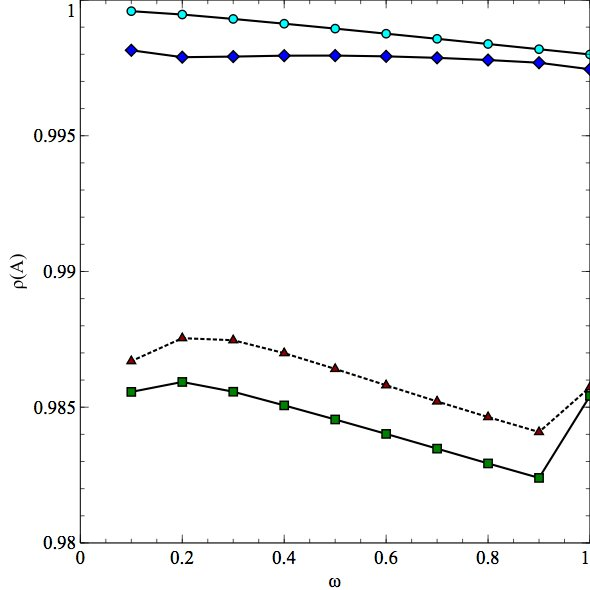
\includegraphics[scale=0.7]{GJplot.jpg}\\
$\blacktriangle$ Gauss-Jacobi Method\\
green (40 iterations, $50\x50$ grid) \\
blue (400 iterations, $50\x50$ grid) \\
cyan (2,000 iterations, $50\x50$ grid)\\
black (40 iterations, $50\x100$ grid)
\end{center}
From the green line (with $50\x50$ grid), we can suggest $\omega = 0.9$ to be the optimal parameter of the Gauss-Jacobi method; by observing the green (40 iterations), blue (400 iterations) and cyan (2,000 iterations) lines, we see the optimal parameter changed from $\omega = 0.9$ to $\omega = 1$ when we increased the iterations. \\
From the red dash line we can see the optimal parameter for a $50\x100$ grid is also $\omega  = 0.9$ (when 40 iterations are used).
\begin{center}
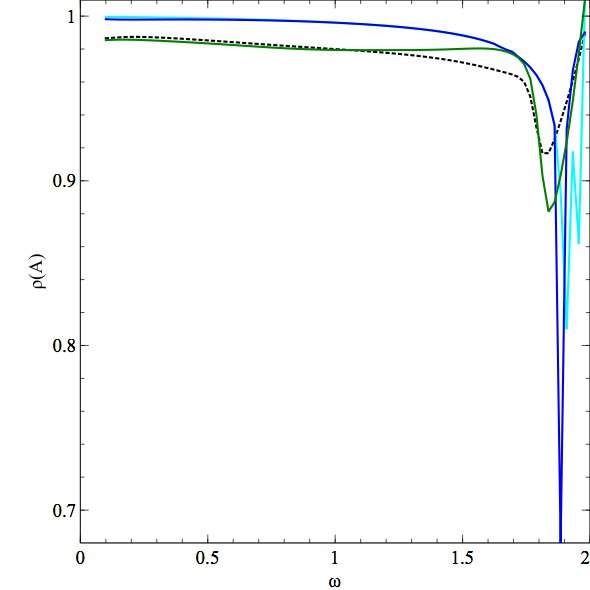
\includegraphics[scale=0.7]{SORplot.jpg} \\
$\blacktriangle$ SOR Method\\
green (40 iterations, $50\x50$ grid) \\
blue (400 iterations, $50\x50$ grid) \\
cyan (2,000 iterations, $50\x50$ grid)\\
black (40 iterations, $50\x100$ grid)\\
\end{center}
(TBH I inspected the .csv file to get the accurate digits for SOR results..) \\
From the green line, we can suggest $\omega = 1.84$ to be the optimal value of the Gauss-Jacobi method; by observing the green (40 iterations), blue (400 iterations) and cyan (2,000 iterations) lines, we see the optimal parameter changed from $\omega = 1.84$ to $\omega = 1.88$ to $\omega = 1.91$ when we increased the iterations from 40 to 400 and to 2,000. \\
From the red dash line we can see the optimal parameter for a $50\x100$ grid is also $\omega  = 1.84$ (when 40 iterations are used).
\end{document}